\chapter{Аппликейшний дэлгэцийн зураглал}
\label{AppendixA}
\pagecolor{white}

Энэ хавсралтад ДЗ-Заал мобайл аппликейшний үндсэн дэлгэцүүдийн screenshot-уудыг харуулав.

%-------------------------------------------------------------------------------

\section*{А.1 Нэвтрэлт ба бүртгэлийн дэлгэц}

\begin{figure}[h]
\centering

\includegraphics[width=0.35\textwidth]{Figures/screenshot_login.png}
\hspace{1cm}

\includegraphics[width=0.35\textwidth]{Figures/screenshot_register.png}
\caption{Нэвтрэх дэлгэц (зүүн) ба бүртгэлийн дэлгэц (баруун)}
\label{fig:screen_auth}
\end{figure}

Email хаяг болон нууц үгээр нэвтрэх дэлгэц нь цайвар бежийн дэвсгэр (\code{\#EDE7DA}) дээр Montserrat фонтоор загварчлагдсан. Бүртгэлийн дэлгэцэд нэр, email, нууц үг оруулах талбарууд байх бөгөөд ``Бүртгүүлэх'' товч дарахад Nodemailer-ийн тусламжтайгаар 6 оронтой баталгаажуулах код илгээгдэнэ.

%-------------------------------------------------------------------------------

\section*{А.2 Нүүр дэлгэц — Спорт заалнуудын жагсаалт}

\begin{figure}[h]
\centering
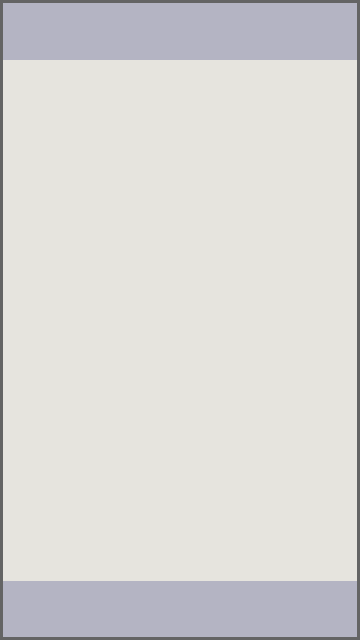
\includegraphics[width=0.35\textwidth]{Figures/screenshot_home.png}
\caption{Нүүр дэлгэц — таван спорт заалны жагсаалт}
\label{fig:screen_home}
\end{figure}

Нүүр дэлгэц нь апп нэвтрэлтийн дараа харагдах анхны дэлгэц юм. Даланзадгадын таван спорт заал картан хэлбэрээр жагсаагдаж, заал бүрийн нэр, байршил, нэг цагийн үнийг харуулна. ``Захиалах'' товч дарахад цагийн хуваарийн дэлгэц нээгдэнэ.

%-------------------------------------------------------------------------------

\section*{А.3 Цагийн хуваарь ба захиалгын дэлгэц}

\begin{figure}[h]
\centering

\includegraphics[width=0.35\textwidth]{Figures/screenshot_booking.png}
\hspace{1cm}

\includegraphics[width=0.35\textwidth]{Figures/screenshot_confirm.png}
\caption{Цагийн хуваарийн дэлгэц (зүүн) ба захиалга баталгаажуулах дэлгэц (баруун)}
\label{fig:screen_booking}
\end{figure}

Цагийн хуваарийн дэлгэцэд сонгосон заал болон огнооны 08:00--00:00 хооронд 16 цагийн үе харагдана. Боломжтой цаг ногоон, захиалагдсан цаг улаан, байгууллагын тогтмол захиалга нил ягаан өнгөөр тэмдэглэгдэнэ. Захиалга баталгаажуулах дэлгэцэд DBK-xxxxx форматын захиалгын код харагдана.

%-------------------------------------------------------------------------------

\section*{А.4 Захиалгын жагсаалт ба AI чатботын дэлгэц}

\begin{figure}[h]
\centering

\includegraphics[width=0.35\textwidth]{Figures/screenshot_bookings.png}
\hspace{1cm}

\includegraphics[width=0.35\textwidth]{Figures/screenshot_chat.png}
\caption{Захиалгын жагсаалтын дэлгэц (зүүн) ба AI чатботын дэлгэц (баруун)}
\label{fig:screen_chat}
\end{figure}

Захиалгын дэлгэцэд хэрэглэгчийн бүх захиалга статусаар (идэвхтэй, дууссан, цуцлагдсан) шүүгдэж харагдана. AI чатботын дэлгэцэд Anthropic Claude Haiku болон Groq Llama загваруудаар дамжуулан спорт заалтай холбоотой асуулт асуух боломжтой.
